\chapter{Experimental Results}
In this final chapter, we will analyze the results of the
models previously described by comparing their respective
training phases, highlighting any issues and strengths of the model.
We will test their performance using the Testing dataset,
as described in Section~\ref{sec:datasetsplitting}, and
evaluate them using various metrics.
Among these metrics, we will employ the MAE (Mean Absolute Error)\cite{metrics}
to highlight the difference between the model's predictions and
the ground truth and the $R^2$ (R-squared)\cite{metrics} index to understand how well
the model-predicted curve approximates the real one.
Here's a brief introduction to the indices we will use:

%In questo ultimo capitolo andremo ad analizzare i risultati dei modelli
%precedentemente descritti confrontando le rispettive fasi di training,
%mettendo in evidenza eventuali problemi e punti di forza del modello.
%Testeremo le perfoance di questi utilizzando il dataset di Testing, descritto
%nella Sezione~\ref{sec:datasetsplitting}, valutandoli impiegando alcune
%metriche come il MAE (Mean Absolute Error) per evidenziare la diferenza tra predizione del modello e la ground turth, e l'indice $R^2$ per capire
%quanto la curva predetta dal modello riesca bene ad approssimare quella reale.
%Di seguito una breve introduzione agli indici che utilizzeremo:

\begin{itemize}
	\item \textbf{Gap MAE}: This metric represents the average pointwise error that the model makes compared to the ground truth. It is expressed in kW.
	      %MAE dell'intero buco, indica in meda l'errore puntuale che il modello commette rispetto alla ground truth. Viene espresso in kW.
	\item \textbf{$R^2$ (R-squared)}: This index quantifies how well the prediction curve approximates the ground truth. It helps us understand how well the model approximates the trend of the reference instant prediction.
	      %$R^2$, questo indice ci va a quantificare quanto bene la curva della predizione approssimi quella della ground truth. Ci permette di
	      %capire quanto bene il modello riesce ad approssimare l'andamento della predizione istantanea di riferimento.
	\item \textbf{Daily MAE}: It is calculated only for individual days within the gap. This metric highlights the average daily error that the model makes, measured in kW.
	      %MAE giornaliero, viene calcolato solo sui singoli giorni del buco. Mette in evidenza l'errore giornaliero medio che commette il modello misurato in kW.
	\item \textbf{Global MAE}: This is the average of all daily errors, expressed in kW.
	      %Global MAE , è la media di tutti i gli errori giornalieri espresso in kW.
	\item \textbf{MAPE (Mean Absolute Percentage Error)}\cite{metrics}: It indicates the error of the model relative to the ground truth, measured in percentage.
	      %MAPE, indica in percentuale quanto è l'errore del modello rispetto la groundh truth, misurato in percentuale
\end{itemize}

\newpage


\section{MLP}\label{sec:mlpbaseline}
In this section, we will introduce the first model, which we will refer to as the
baseline model, based on a Multi-Layer Perceptron.
We will analyze its architecture, the training phase, and its final performance.

%In questa sezione andremo ad introdurre il primo modello a cui faremo
%riferiento come baseline model, basato su MultiLayer Perceptron.
%Analizzeremo la sua architettura, la 
%fase di training e le sue performance finali.

\subsection{Architecture}
This neural network is designed to predict the instantaneous energy output over
a period of exactly 2 days.
To do this, it requires input data that includes the performance of the system
(features selected during the Preprocessing phase, see Chapter \ref{chap:datapreprocessing}) for exactly one day
before and one day after the period in question.
This enables it to understand how the system is performing and,
consequently, provide the energy output trend.
The model consists of 6 main layers:

%Questa rete neurale è progettata per prevedere l'andamento dell'energia istantanea prodotta durante un periodo di un buco di esattamente 2 giorni.
%Per farlo ha bisogno di avere come input l'andamento dell'impianto (features selezionate nella fase di preprocessing) di esattamente un giorno prima del
%buco e di un giorno dopo. In questo modo può riuscire a comprendere come l'impianto sta performando e quindi restituire l'andamento dell'energia.
%Il modello è formato da 6 livelli principali:

\begin{figure}[H]
	\begin{minipage}{0.6\textwidth}
		\begin{itemize}
			\item \textbf{Input layer}: This is the first layer of the network.
			      It takes two input tensors: \textit{before} and \textit{after}.
			      These tensors represent the day before and the day after the specific period we want to
			      predict. They have the shape \verb|[BATCH_SIZE, 96, 33]|, where 96 is the number
			      of timestamps in our dataset that make up one day, and 33 represents the
			      features obtained from the Data Preprocessing phase.
			      These tensors are then flattened and concatenated to be passed to the subsequent layer.
			      The output of this layer goes through a Batch Normalization layer, and the
			      Rectified Linear Unit (ReLU) activation function is used.

			      % è il primo livello della rete, prende in input 2 tensori: \textit{before} e \textit{after}. Questi stanno ad indicare rispettivamente il giorno prima e quello dopo del buco che vogliamo chiudere. Avranno la forma \verb|[BATCH_SIZE, 96, 33]|, dove \verb|96| è il numero di timestamp del nostro dataset che formano un giorno e \verb|33| sono le feature ottenute dalla fase di preprocessing dei dati. A questi verrà poi applicata un'operazione di Flatten ed infine concatenati per poter essere poi passati al layer successio.
			      %L'output di questo layer passa per un livello di Batch Normalization e viene utilizzata la ReLu come funzione di attivazione. 

			\item \textbf{Hidden layers}: In total, there are 4 layers, each of which takes the
			      output of the previous layer as input and reduces the number of neurons by half.
			      Batch Normalization is applied to the result, and the Rectified Linear Unit (ReLU)
			      is used as the activation function.

			      %in totale 4, ognuno prende in input il risultato del layer precedente e va a dimezzare il numero dei neuroni. Al risultato viene applicata un'operazione di Batch Normalization e utilizzata la ReLu come funzione di attivazione.

			\item \textbf{Output layer}: The final layer of our network, it takes the result from the
			      previous layer and outputs the value of the Instantaneous Energy Produced
			      during the specific period.
			      It produces a tensor with a shape of \verb|[BATCH_SIZE, 192, 1]|.
			      The SoftPlus function is used as the final activation function.

			      %ultimo layer della nostra rete, dal risultato del layer precedente riporta come output il valore dell'Energia Istantanea Prodotta durante il buco, un tensore di forma \verb|[BATCH_SIZE, 192, 1]|. Viene utilizzata la SoftPlus come funzione di attivazione finale.
		\end{itemize}
	\end{minipage}%
	\hspace{0.5cm}
	\begin{minipage}{0.4\textwidth}
		\centering
		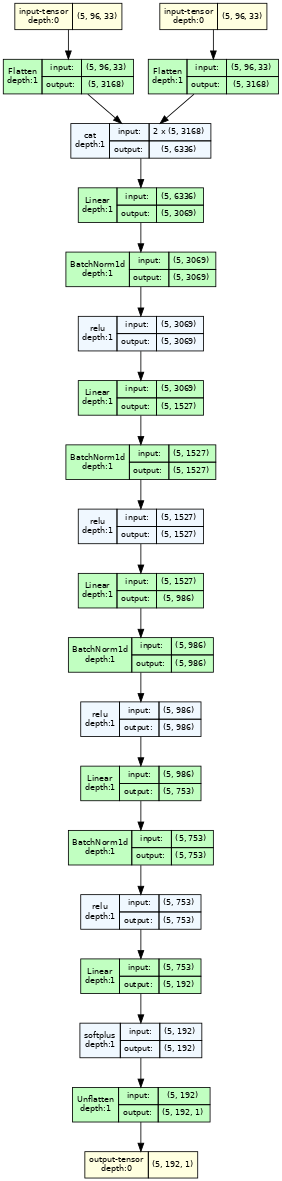
\includegraphics[width=0.5\textwidth]{chapters/3_models/imgs/ufcnmodel.png}
		\caption{Beseline Model architecture visualization.}\label{fig:baselinemodelarch}
	\end{minipage}
\end{figure}

\begin{minipage}[t]{0.5\textwidth}
	\begin{figure}[H]
		\centering
		\begin{tikzpicture}
			\draw[->] (-3,0) -- (3,0) node[right] {$x$};
			\draw[->] (0,-1) -- (0,4) node[above] {$y$};
			\draw[dotted] (-3,-1) grid (3,4);
			\draw[color=blue, domain=-3:0] plot[id=logistic] function{0};
			\draw[color=blue, domain=0:3] plot[id=logistic] function{x};
		\end{tikzpicture}
		\caption{Rectified Linear Unit function. $ReLu(x) = \max(0, x)$}
		\label{fig:relu}
	\end{figure}
\end{minipage}%
\hspace{.5cm}
\begin{minipage}[t]{0.5\textwidth}
	\begin{figure}[H]
		\centering
		\begin{tikzpicture}
			\draw[->] (-3,0) -- (3,0) node[right] {$x$};
			\draw[->] (0,-1) -- (0,4) node[above] {$y$};
			\draw[dotted] (-3,-1) grid (3,4);
			\draw[color=blue, domain=-3:3] plot[id=logistic] function{log(1+exp(x))};
		\end{tikzpicture}
		\caption{SoftPlus function. $SoftPlus(x) = \frac{1}{\beta} \log(1+e^{\beta x})$}
		\label{fig:softplus}
	\end{figure}
\end{minipage}

\subsection{Training}
The model was trained by artificially creating gaps of two days in length within the
training dataset.
These gaps were passed to the network in the format described earlier,
and the output result was compared to the actual instantaneous energy produced during the gap.
An \textit{Early Stopping} procedure was implemented to prevent training from continuing if
the model was not improving its performance.
A procedure, called \textit{Save Best}, has also been integrated,
which saves the model to a file whenever the Validation Loss improves.
The validation dataset was applied in this phase to assess the learning progress at the end
of each epoch.
A normalization procedure of the area was applied to the model's output in relation to
that of the gap to ensure that the output starts exactly from the last value of the
instantaneous energy produced \textit{before} and ends exactly with the first value
of the energy produced \textit{after}. Adam was used as the optimizer,
and L1Loss (Equation~\ref{eq:l1loss}) served as the loss function.
We chose to set the batch size parameter to 10, the learning rate $\lambda$ to 0.01,
a maximum of 100 epochs, and a patience value of 20 for Early Stopping.

%Il modello è stato allenato creando, in modo artificiale, buchi di lunghezza
%pari a due giorni all'interno del dataset di training, passati alla rete nel formato
%descritto precedentemente e confrontato il risultato in output con l'effettiva energia istantanea
%prodotta del buco. \'{E} stata implementata una procedura di \textit{Early Stopping} per evitare
%di continuare l'allenamento anche se il modello non sta migliorando le sue performance. 
%\'{E} stata anche integrata una procedura, chiamata \textit{Save Best},
%che salva il modello su file ogni qualvolta la validation loss migliori.
%Il dataset di validation è stato applicato in questa fase per verificare lo stato di
%apprendimento alla fine di ogni epoca. All'output del modello è stata applicata una 
%procedura di normalizzazione dell'area rispetto a quella del buco per far si che la predizione
%parta esattamente dall'ultimo valore dell' energia istantanea prodotta di \textit{before} e
%termini esattamente con il primo valore di \textit{after}.
%\'{E} stato impiegato Adam come ottimizzatore e la L1Loss (Equation \ref{eq:l1loss}) come loss function.
%Abbiamo scelto di impostare il parametro batch size a 10, learning rate $\lambda$ a 0.01, 100
%come numero massimo di epoche e 20 come patience per l'Early Stopping.

\begin{gather}\label{eq:l1loss}
	L = \{l_1,\dots,l_N\}^\top, \quad
	l_n = \left| x_n - y_n \right|,\\
	\ell(x,y) = \operatorname{mean}(L)
\end{gather}

\begin{table}[H]
	\begin{center}
		\begin{tabular}[c]{l|l}

			\textbf{Total Parameters (\#)}     & 26543400 \\
			\textbf{Trainable Parameters (\#)} & 26543400 \\
			\textbf{Training Duration (s)}     & 24.0     \\
			\textbf{Model Size (MB)}           & 101.3
		\end{tabular}
	\end{center}
	\caption{Baseline Model specification.}\label{tab:ufcnspecs}
\end{table}

\begin{figure}[H]
	\centering
	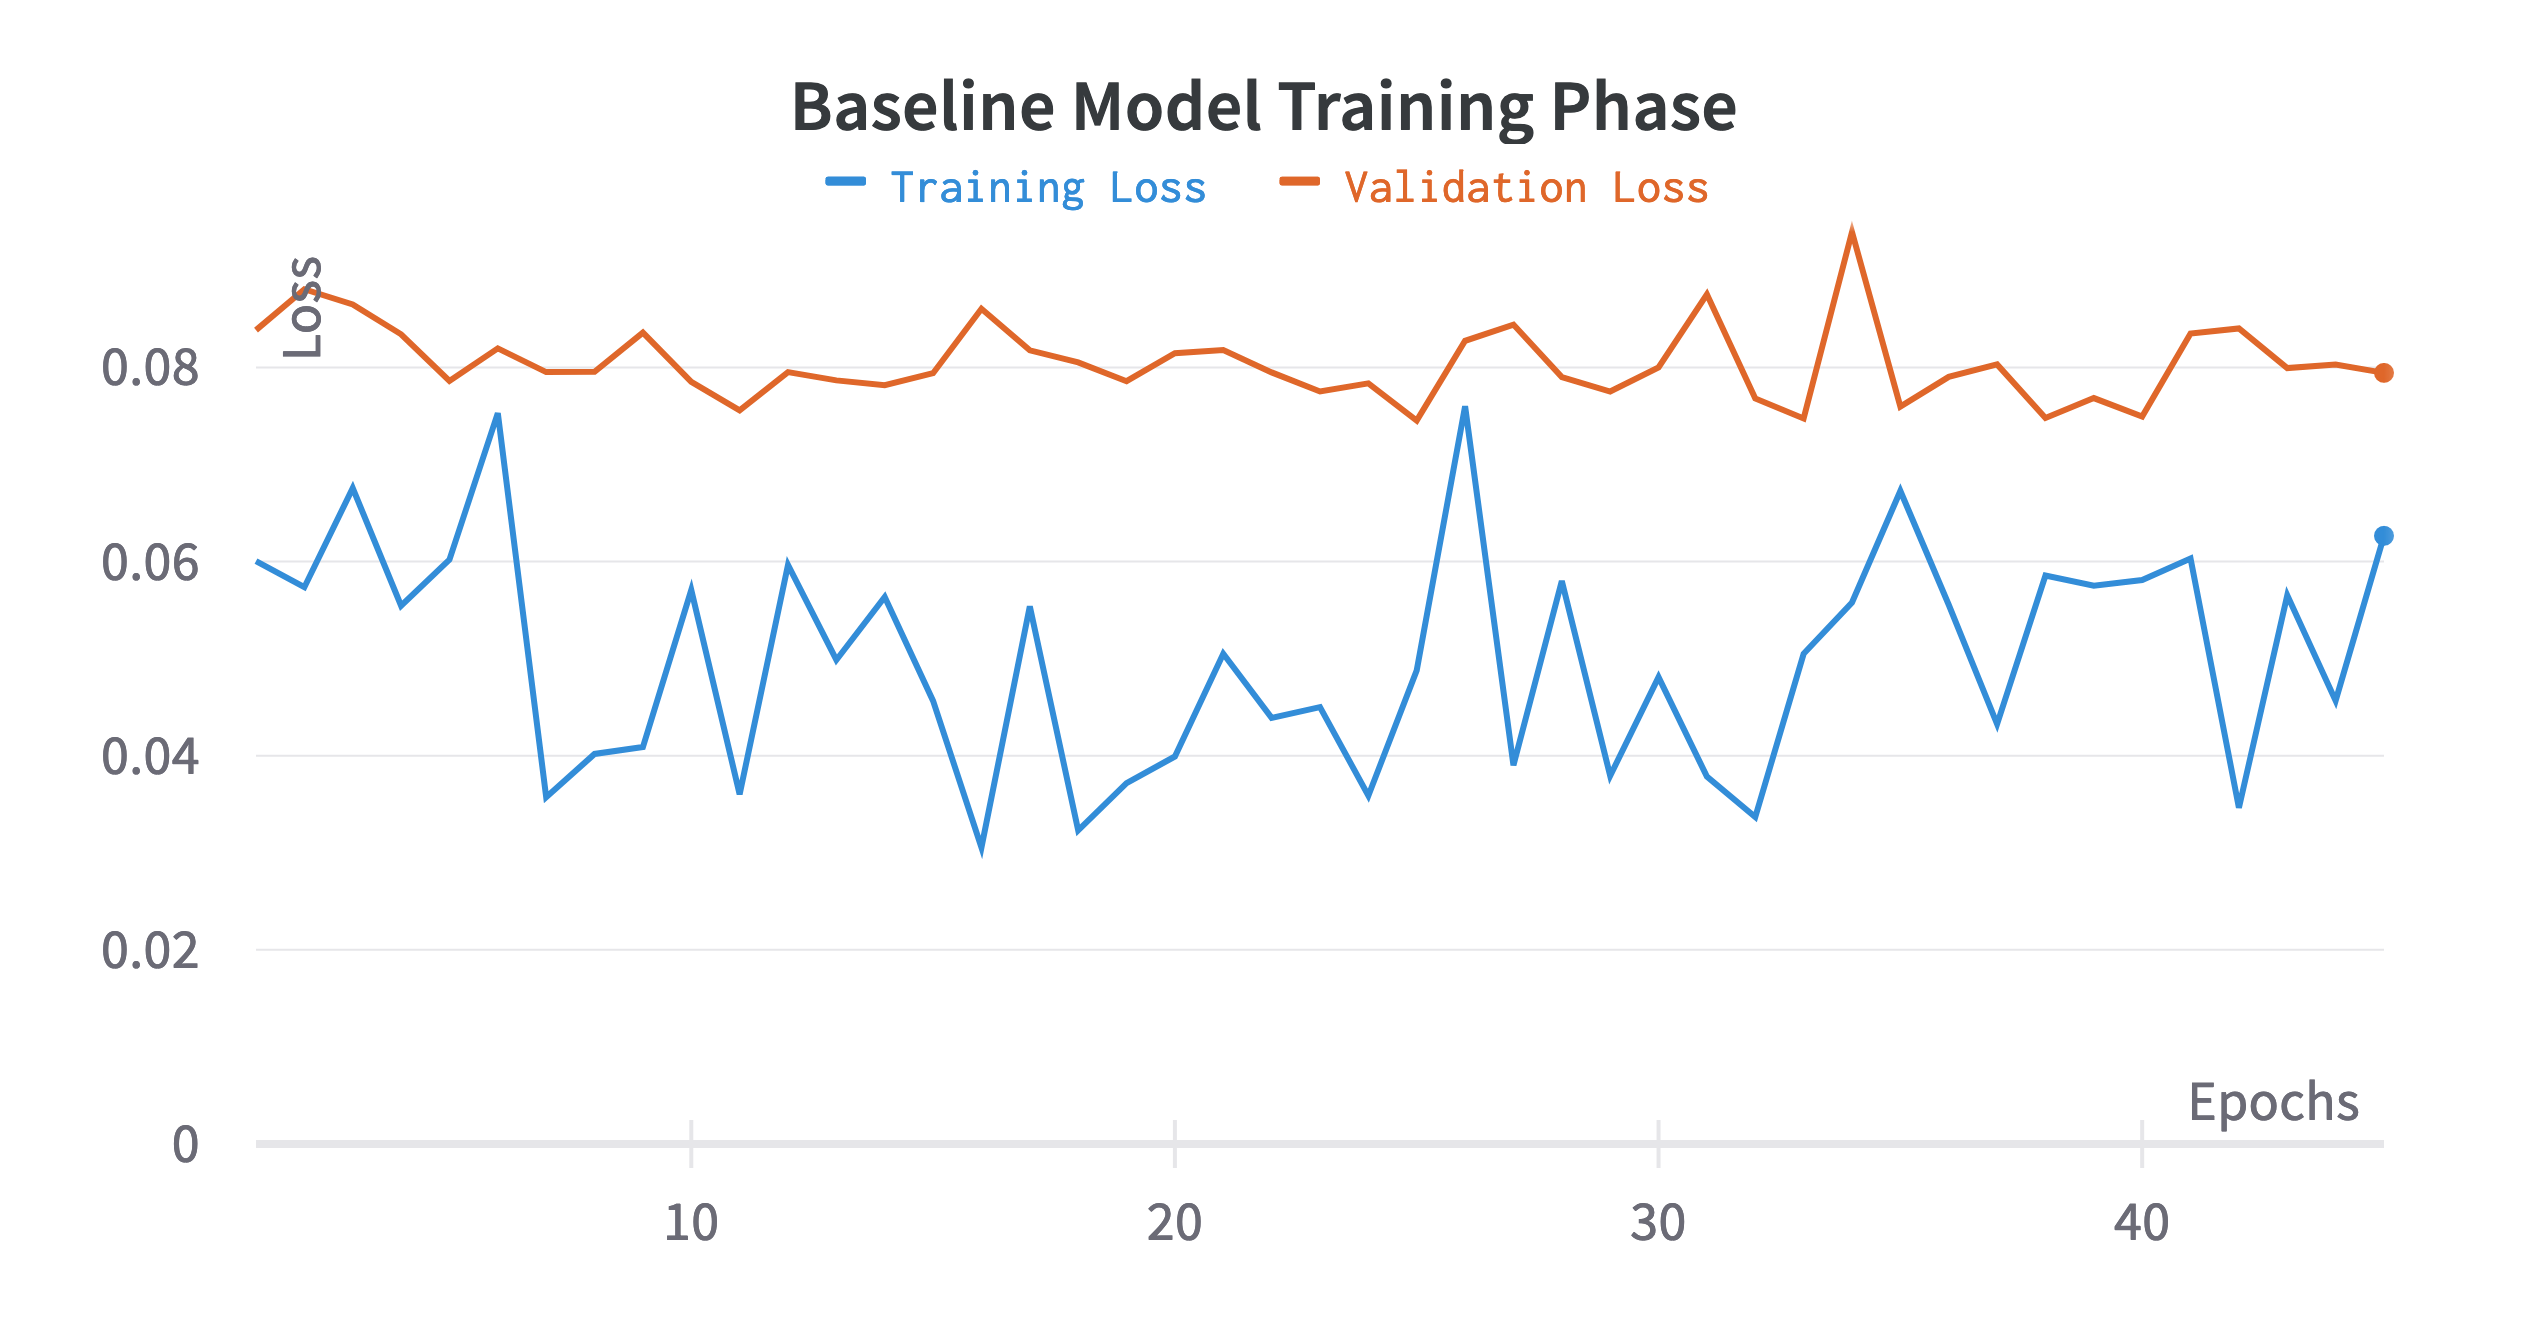
\includegraphics[width=\textwidth]{chapters/3_models/imgs/ufnc/ufnctraining.png}
	\caption{The chart displays the loss progression during the training phase. The blue line represents the Training Loss, while the orange line represents the Validation Loss.}
	\label{fig:ufcntraining}
\end{figure}

\begin{figure}[H]
	\centering
	\begin{subfigure}{0.32\textwidth}
		\centering
		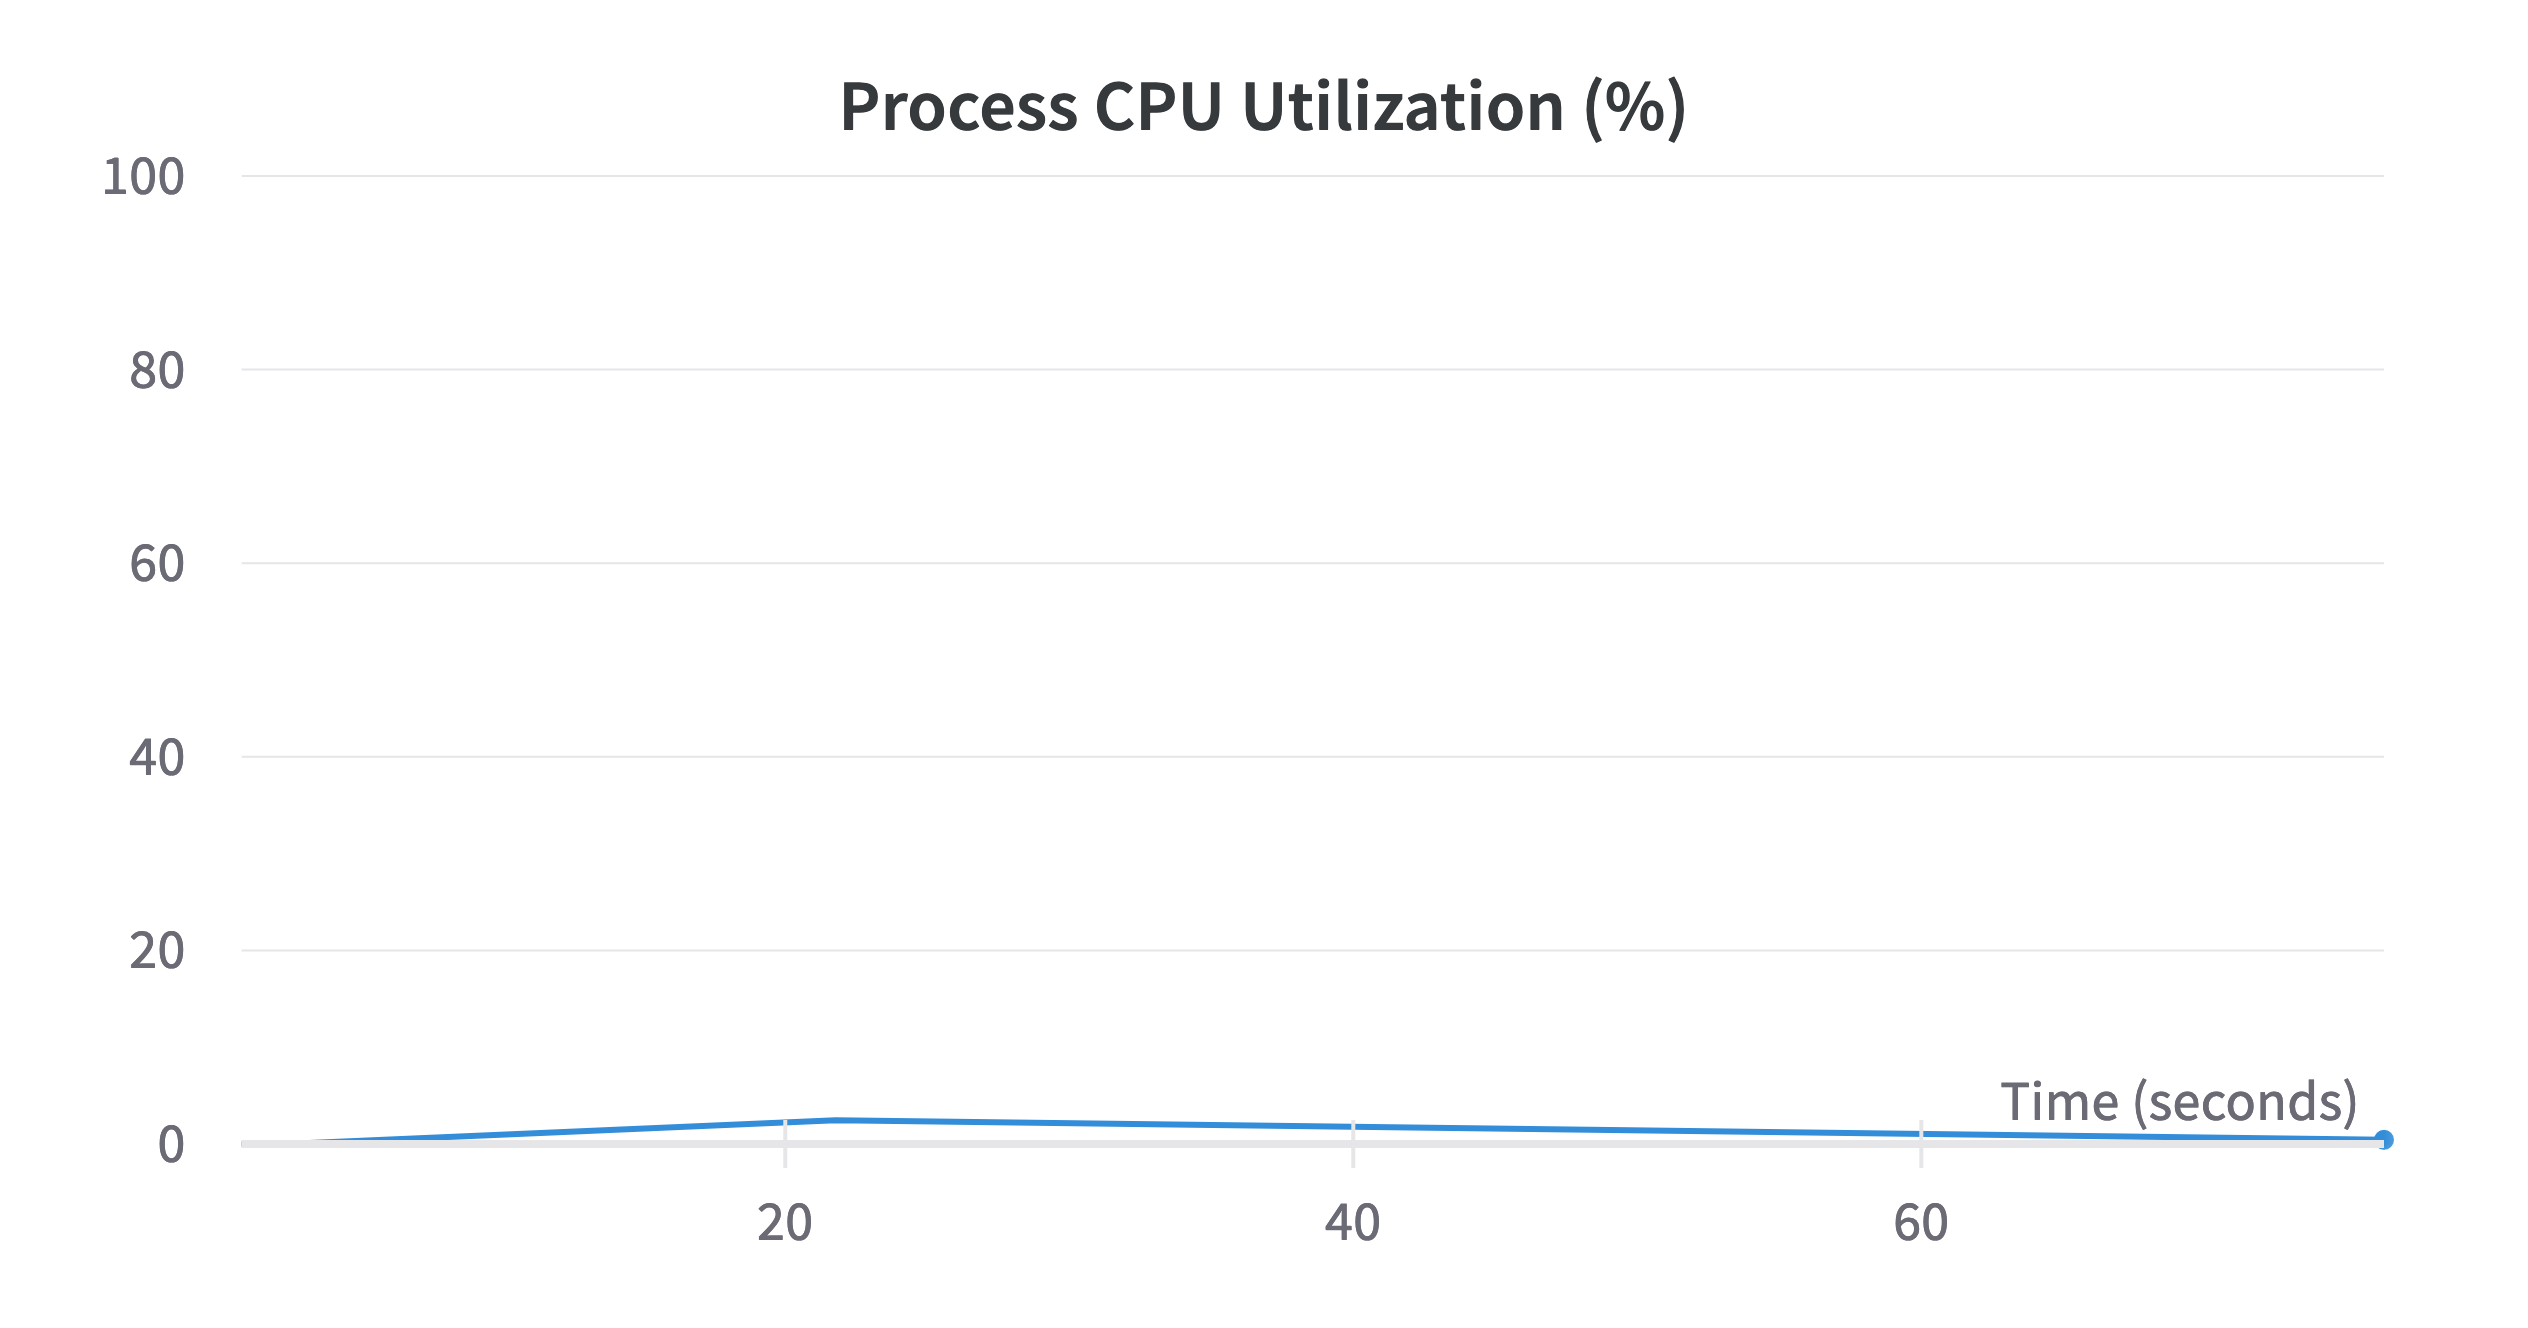
\includegraphics[width=\textwidth]{chapters/3_models/imgs/ufnc/ufcncpusage.png}
	\end{subfigure}
	\begin{subfigure}{0.32\textwidth}
		\centering
		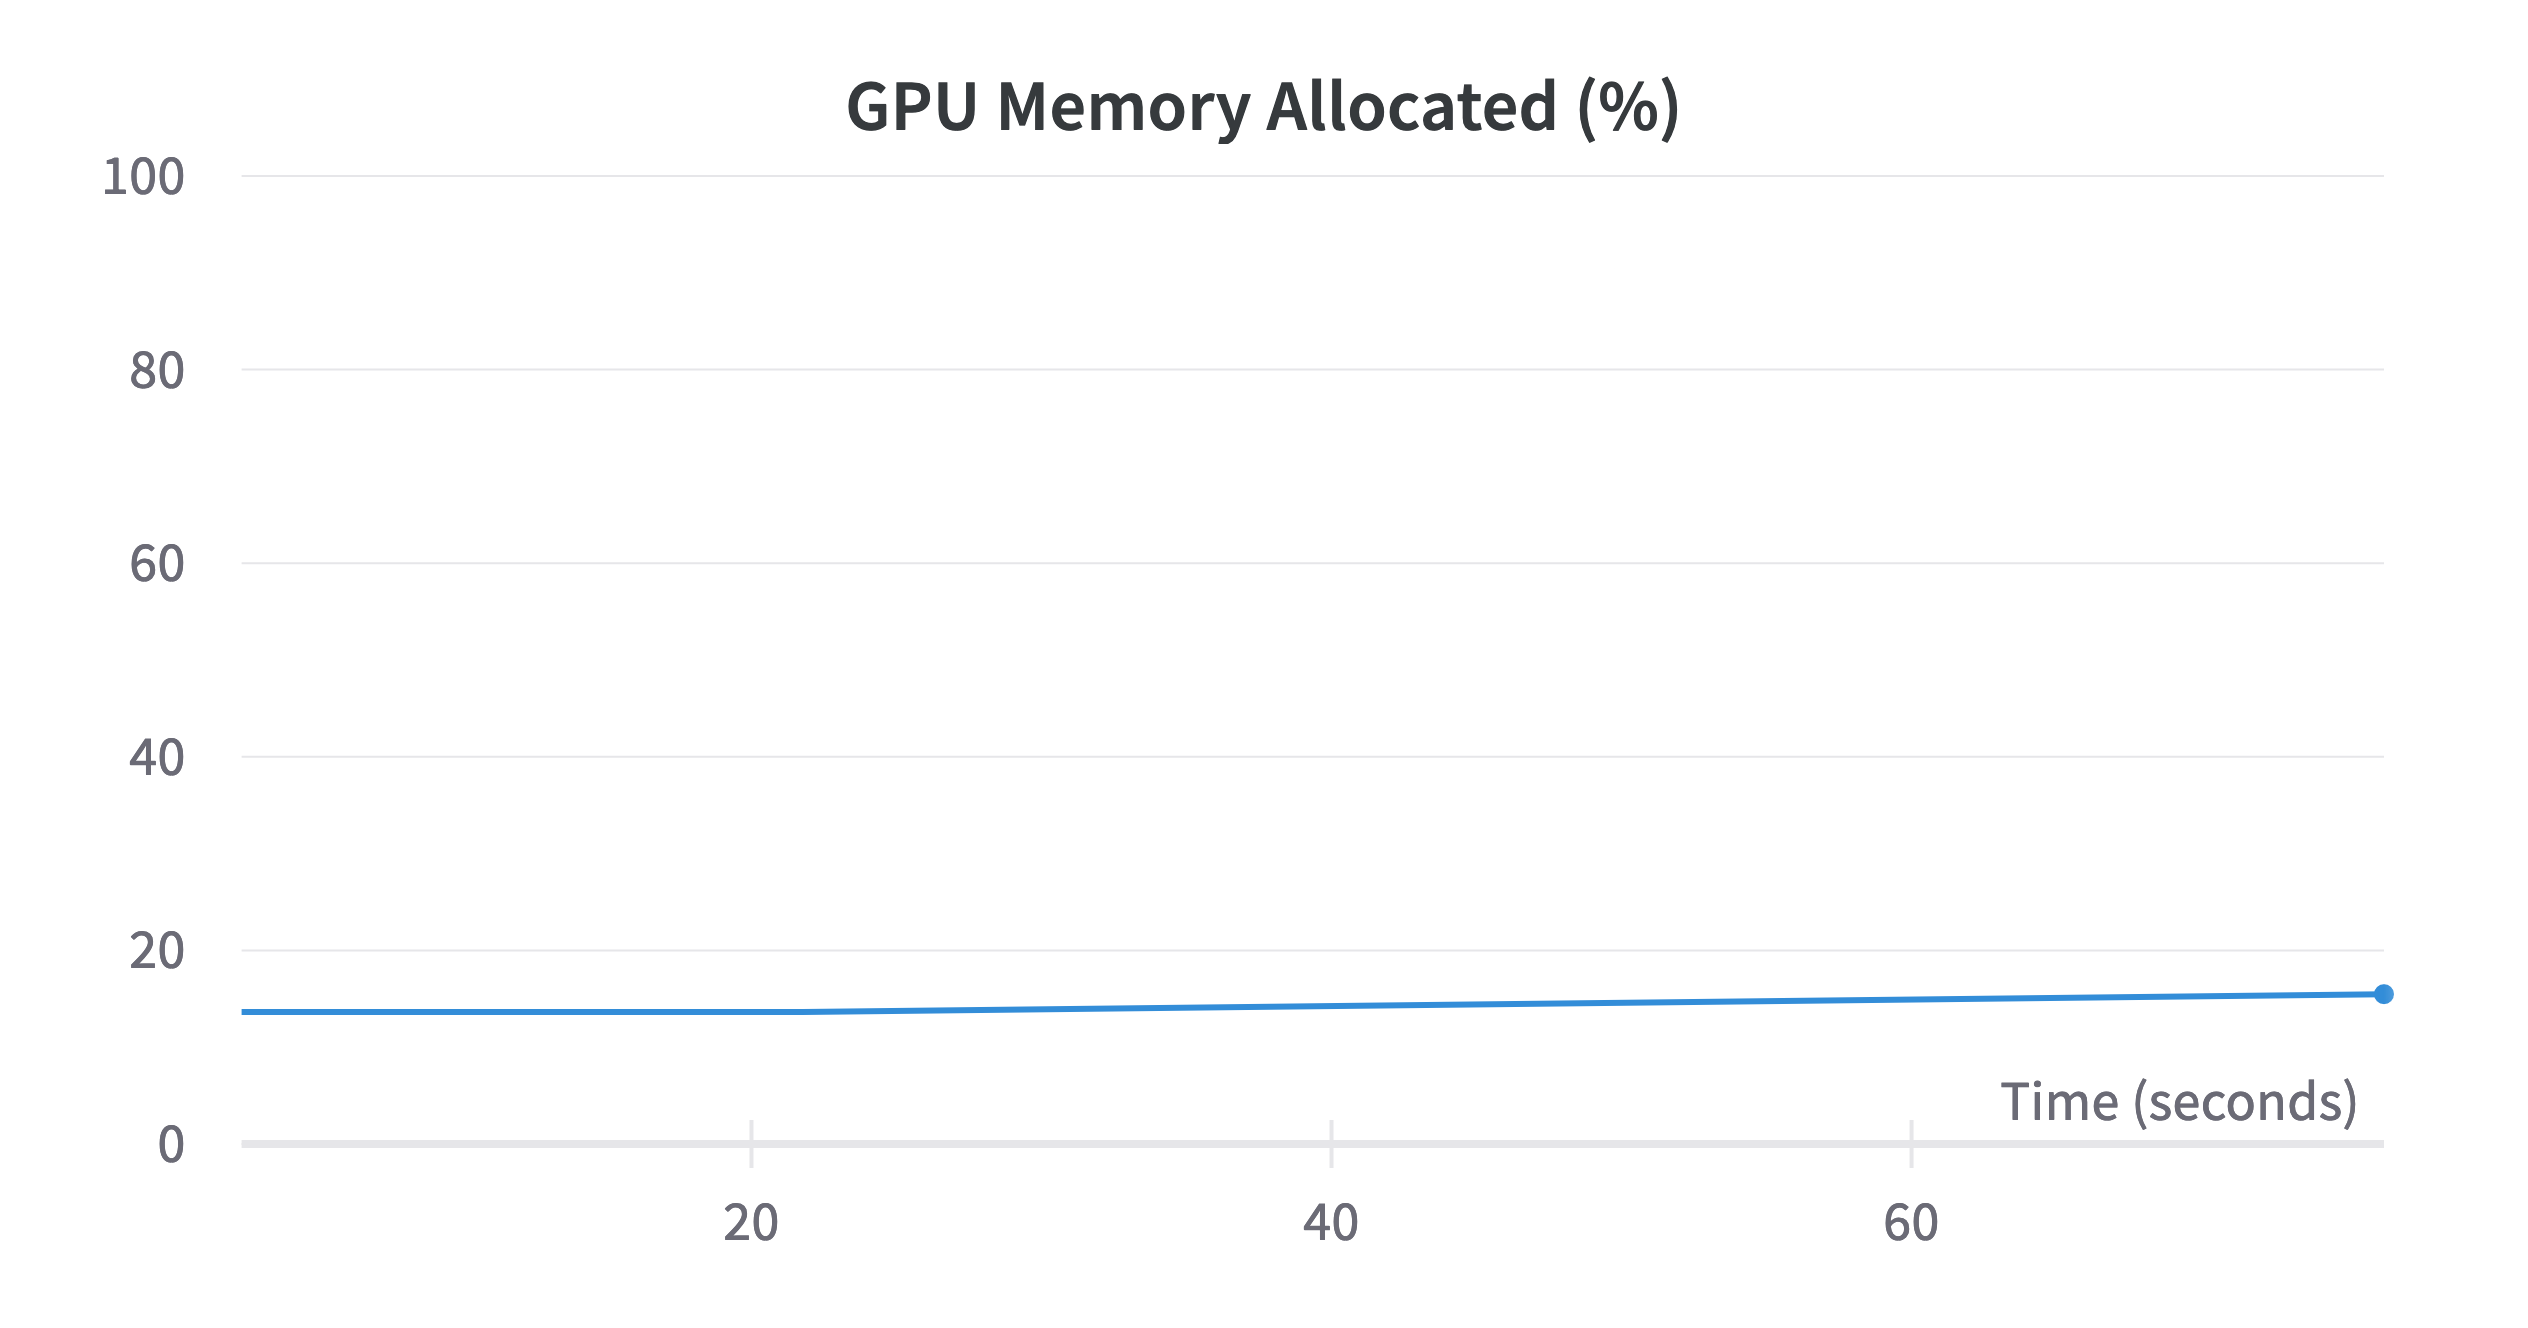
\includegraphics[width=\textwidth]{chapters/3_models/imgs/ufnc/ufcnmem.png}
	\end{subfigure}
	\begin{subfigure}{0.32\textwidth}
		\centering
		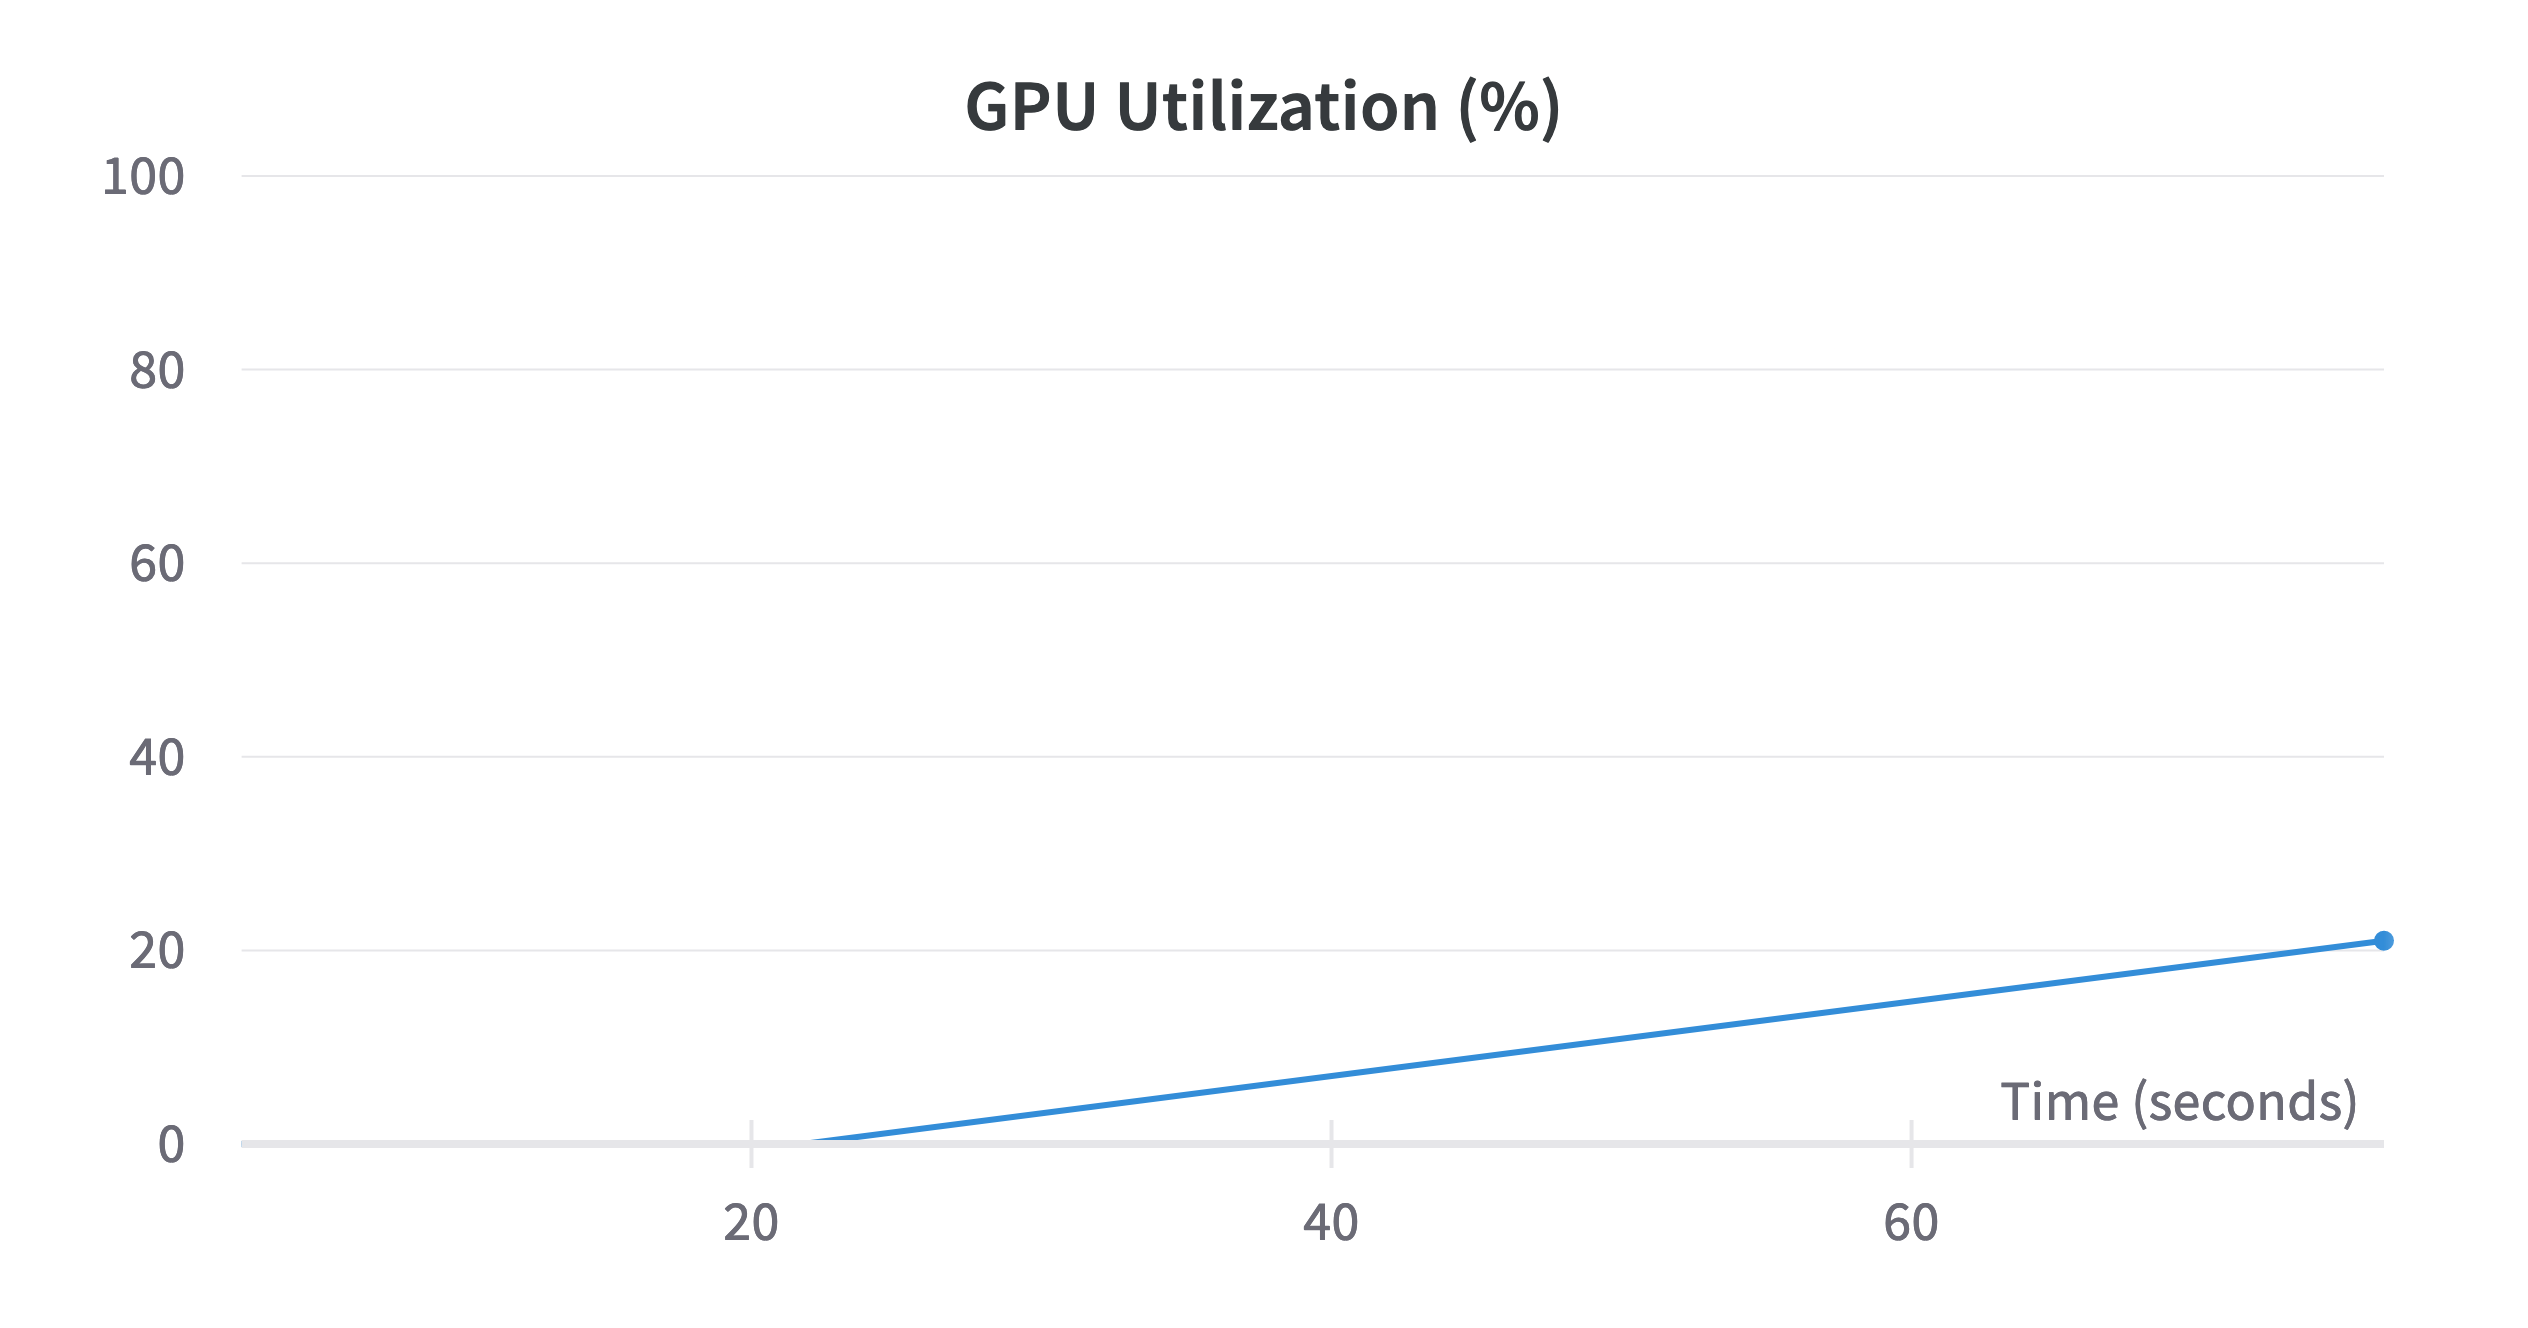
\includegraphics[width=\textwidth]{chapters/3_models/imgs/ufnc/ufcnusagevera.png}
	\end{subfigure}\\
	\begin{subfigure}{0.32\textwidth}
		\centering
		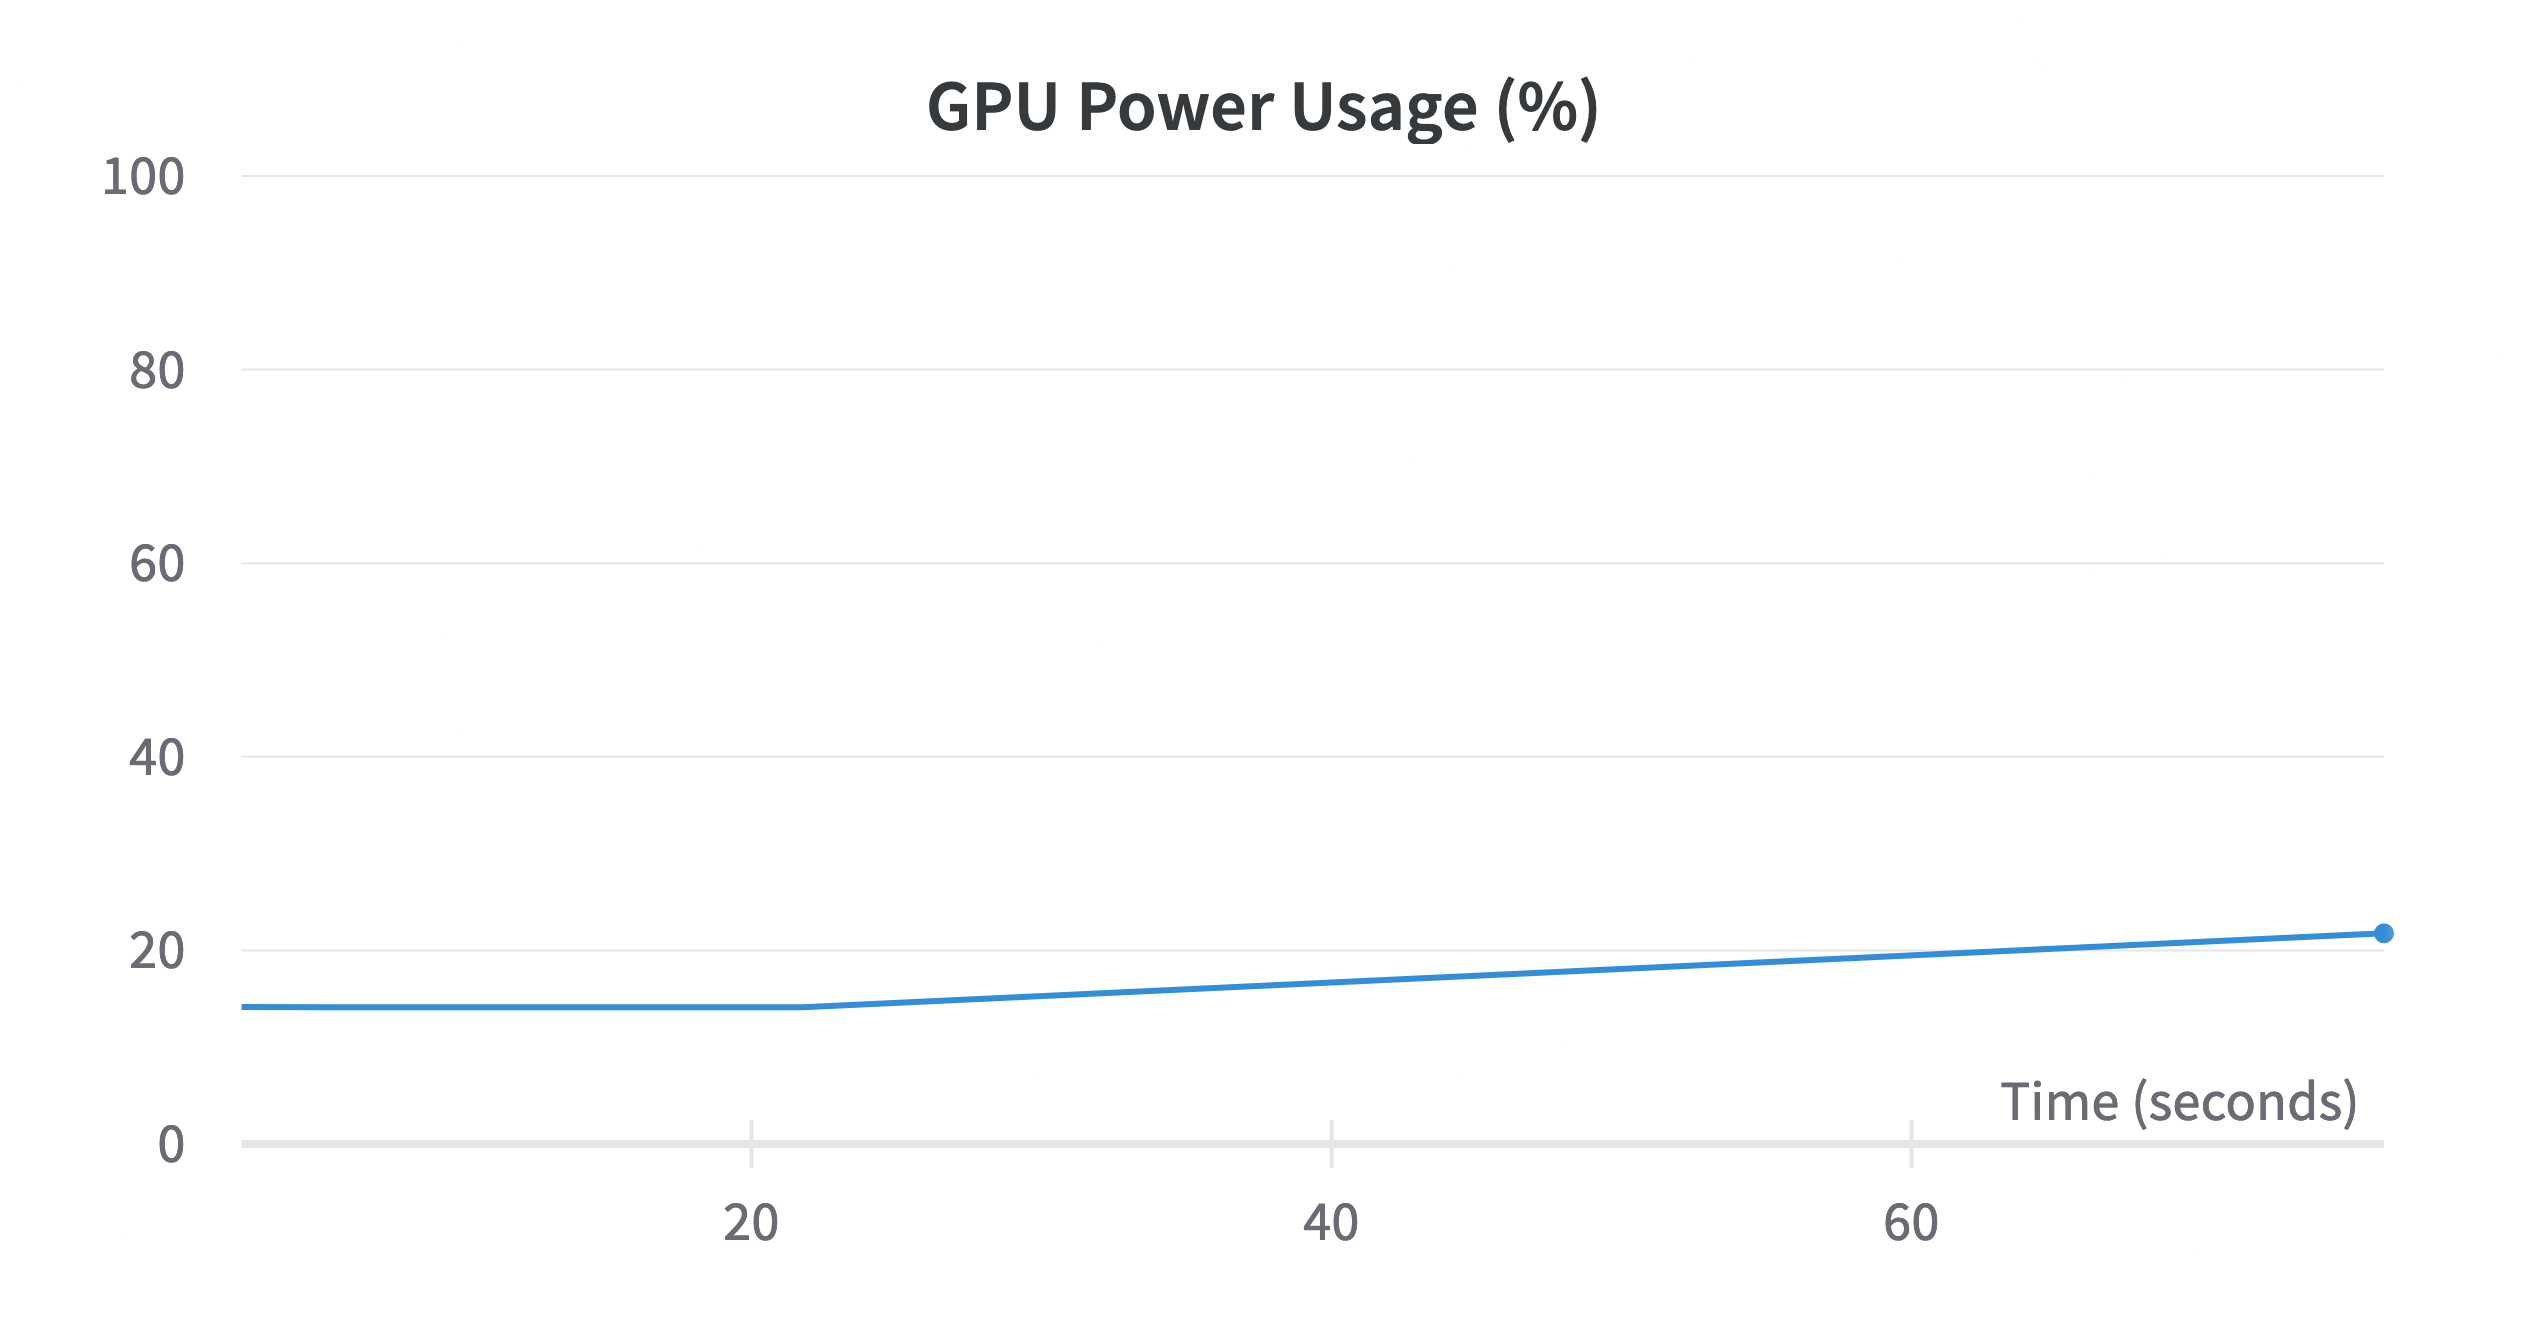
\includegraphics[width=\textwidth]{chapters/3_models/imgs/ufnc/ufncusageperc.png}
	\end{subfigure}
	\begin{subfigure}{0.32\textwidth}
		\centering
		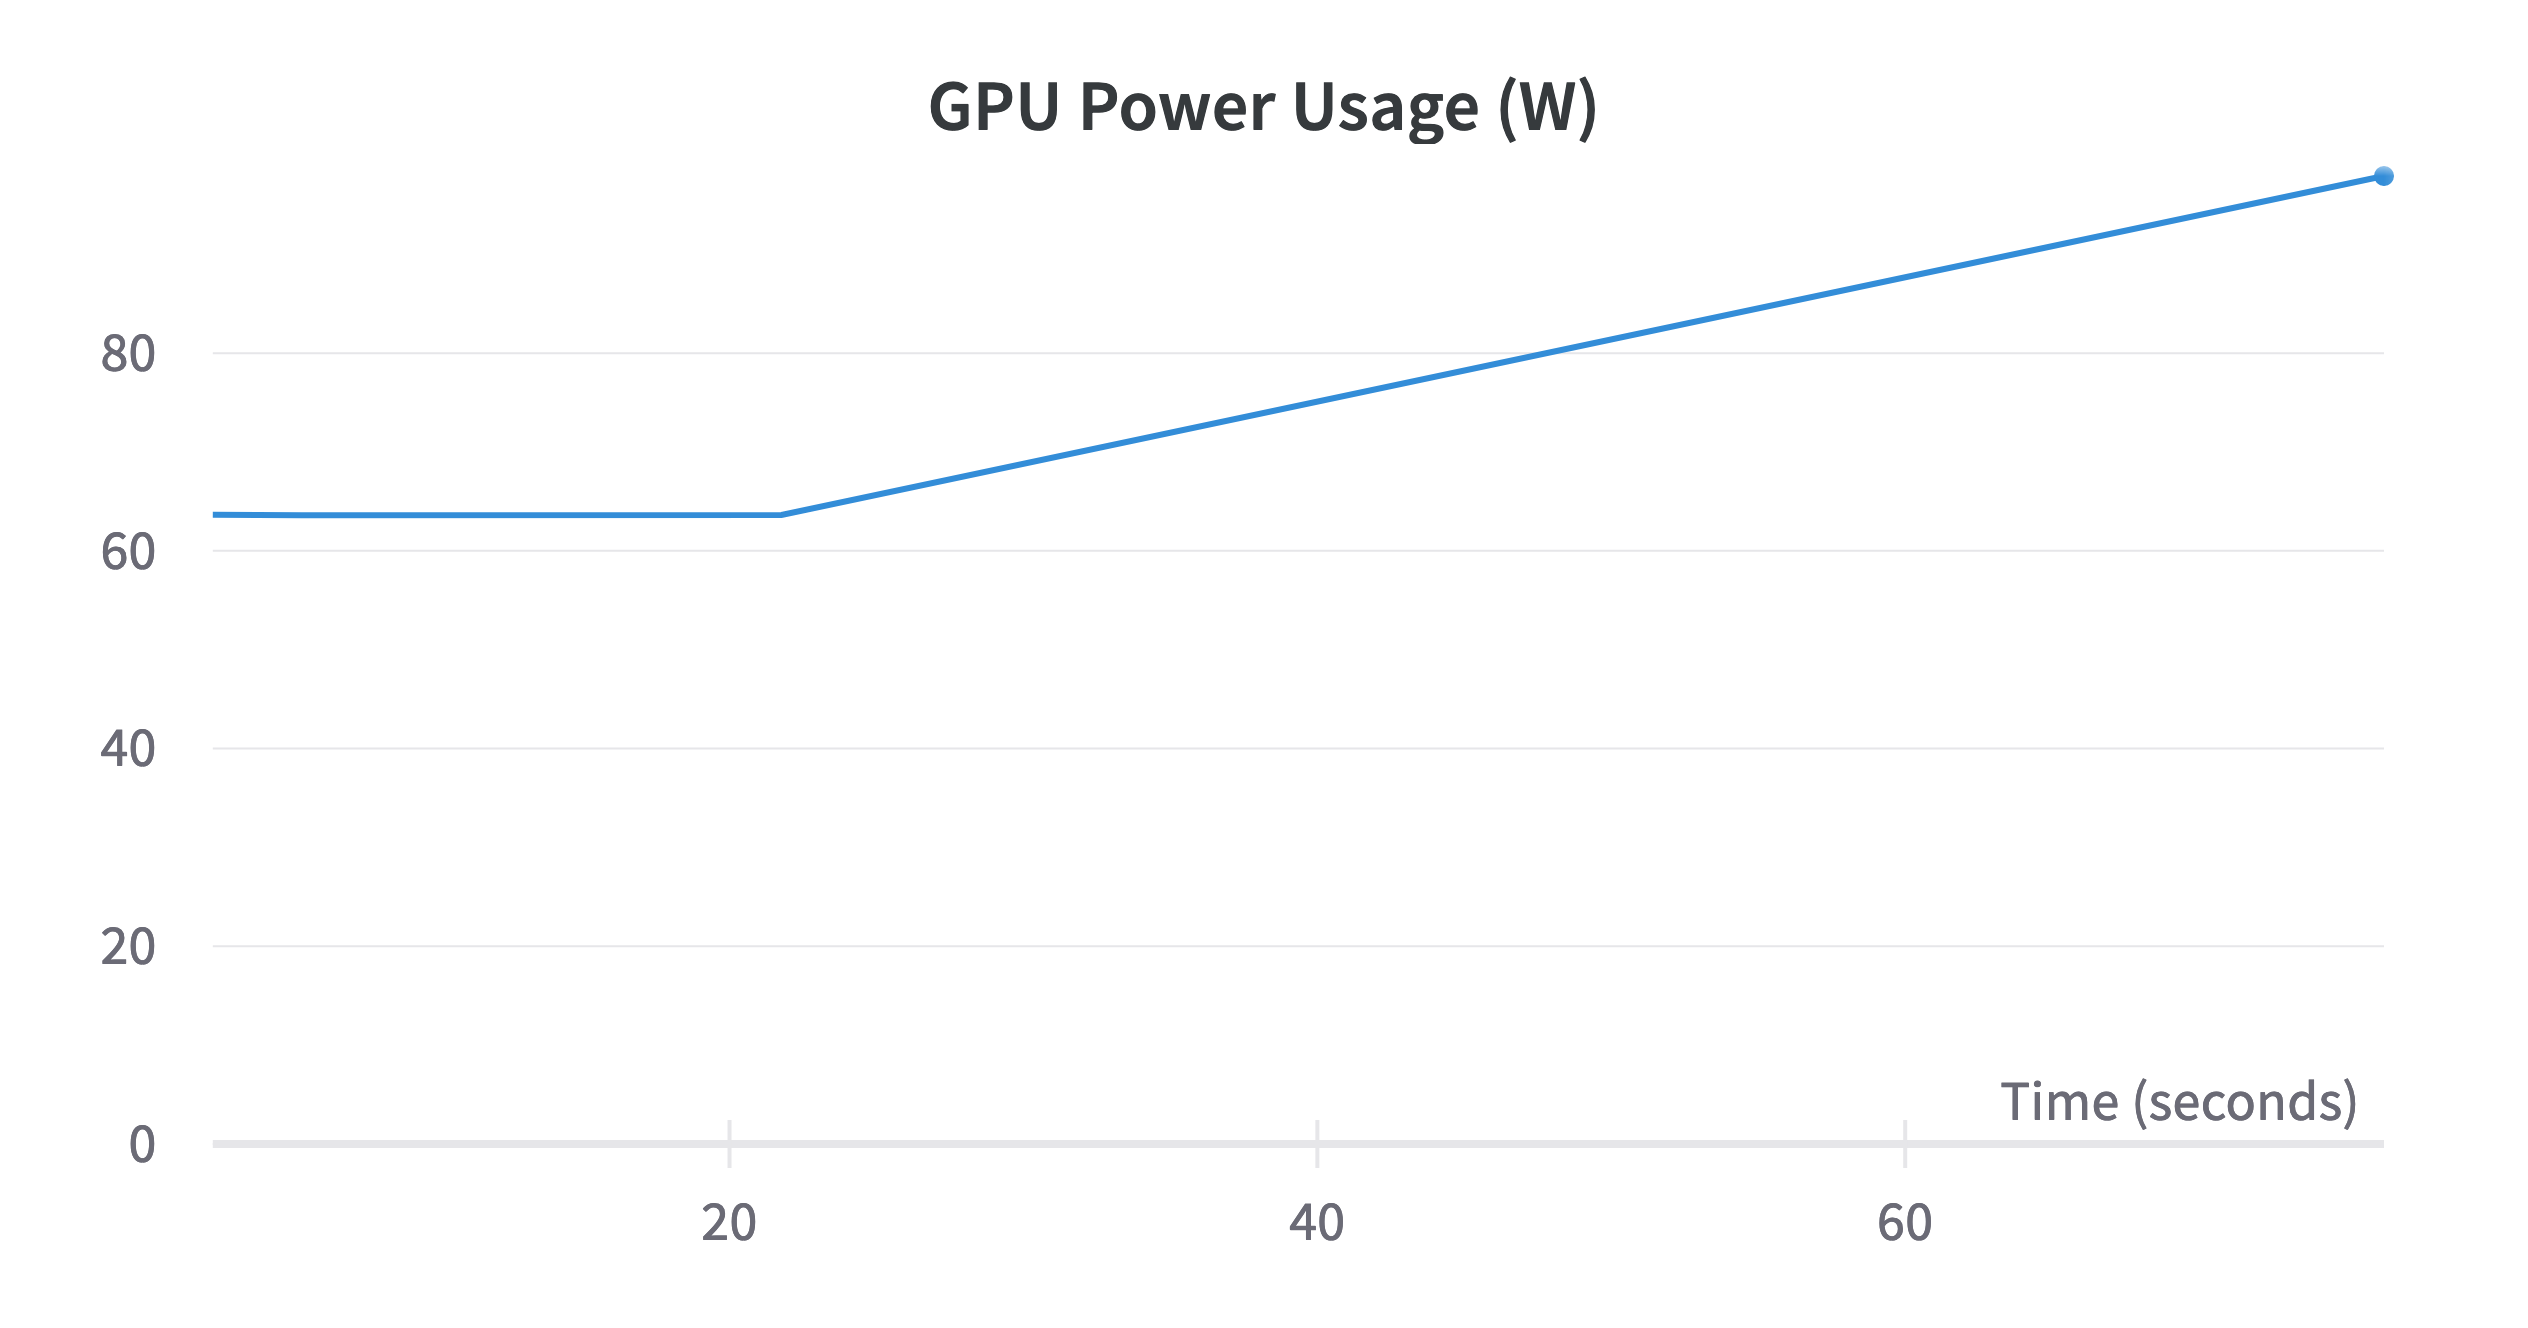
\includegraphics[width=\textwidth]{chapters/3_models/imgs/ufnc/ufncusagew.png}
	\end{subfigure}
	\begin{subfigure}{0.32\textwidth}
		\centering
		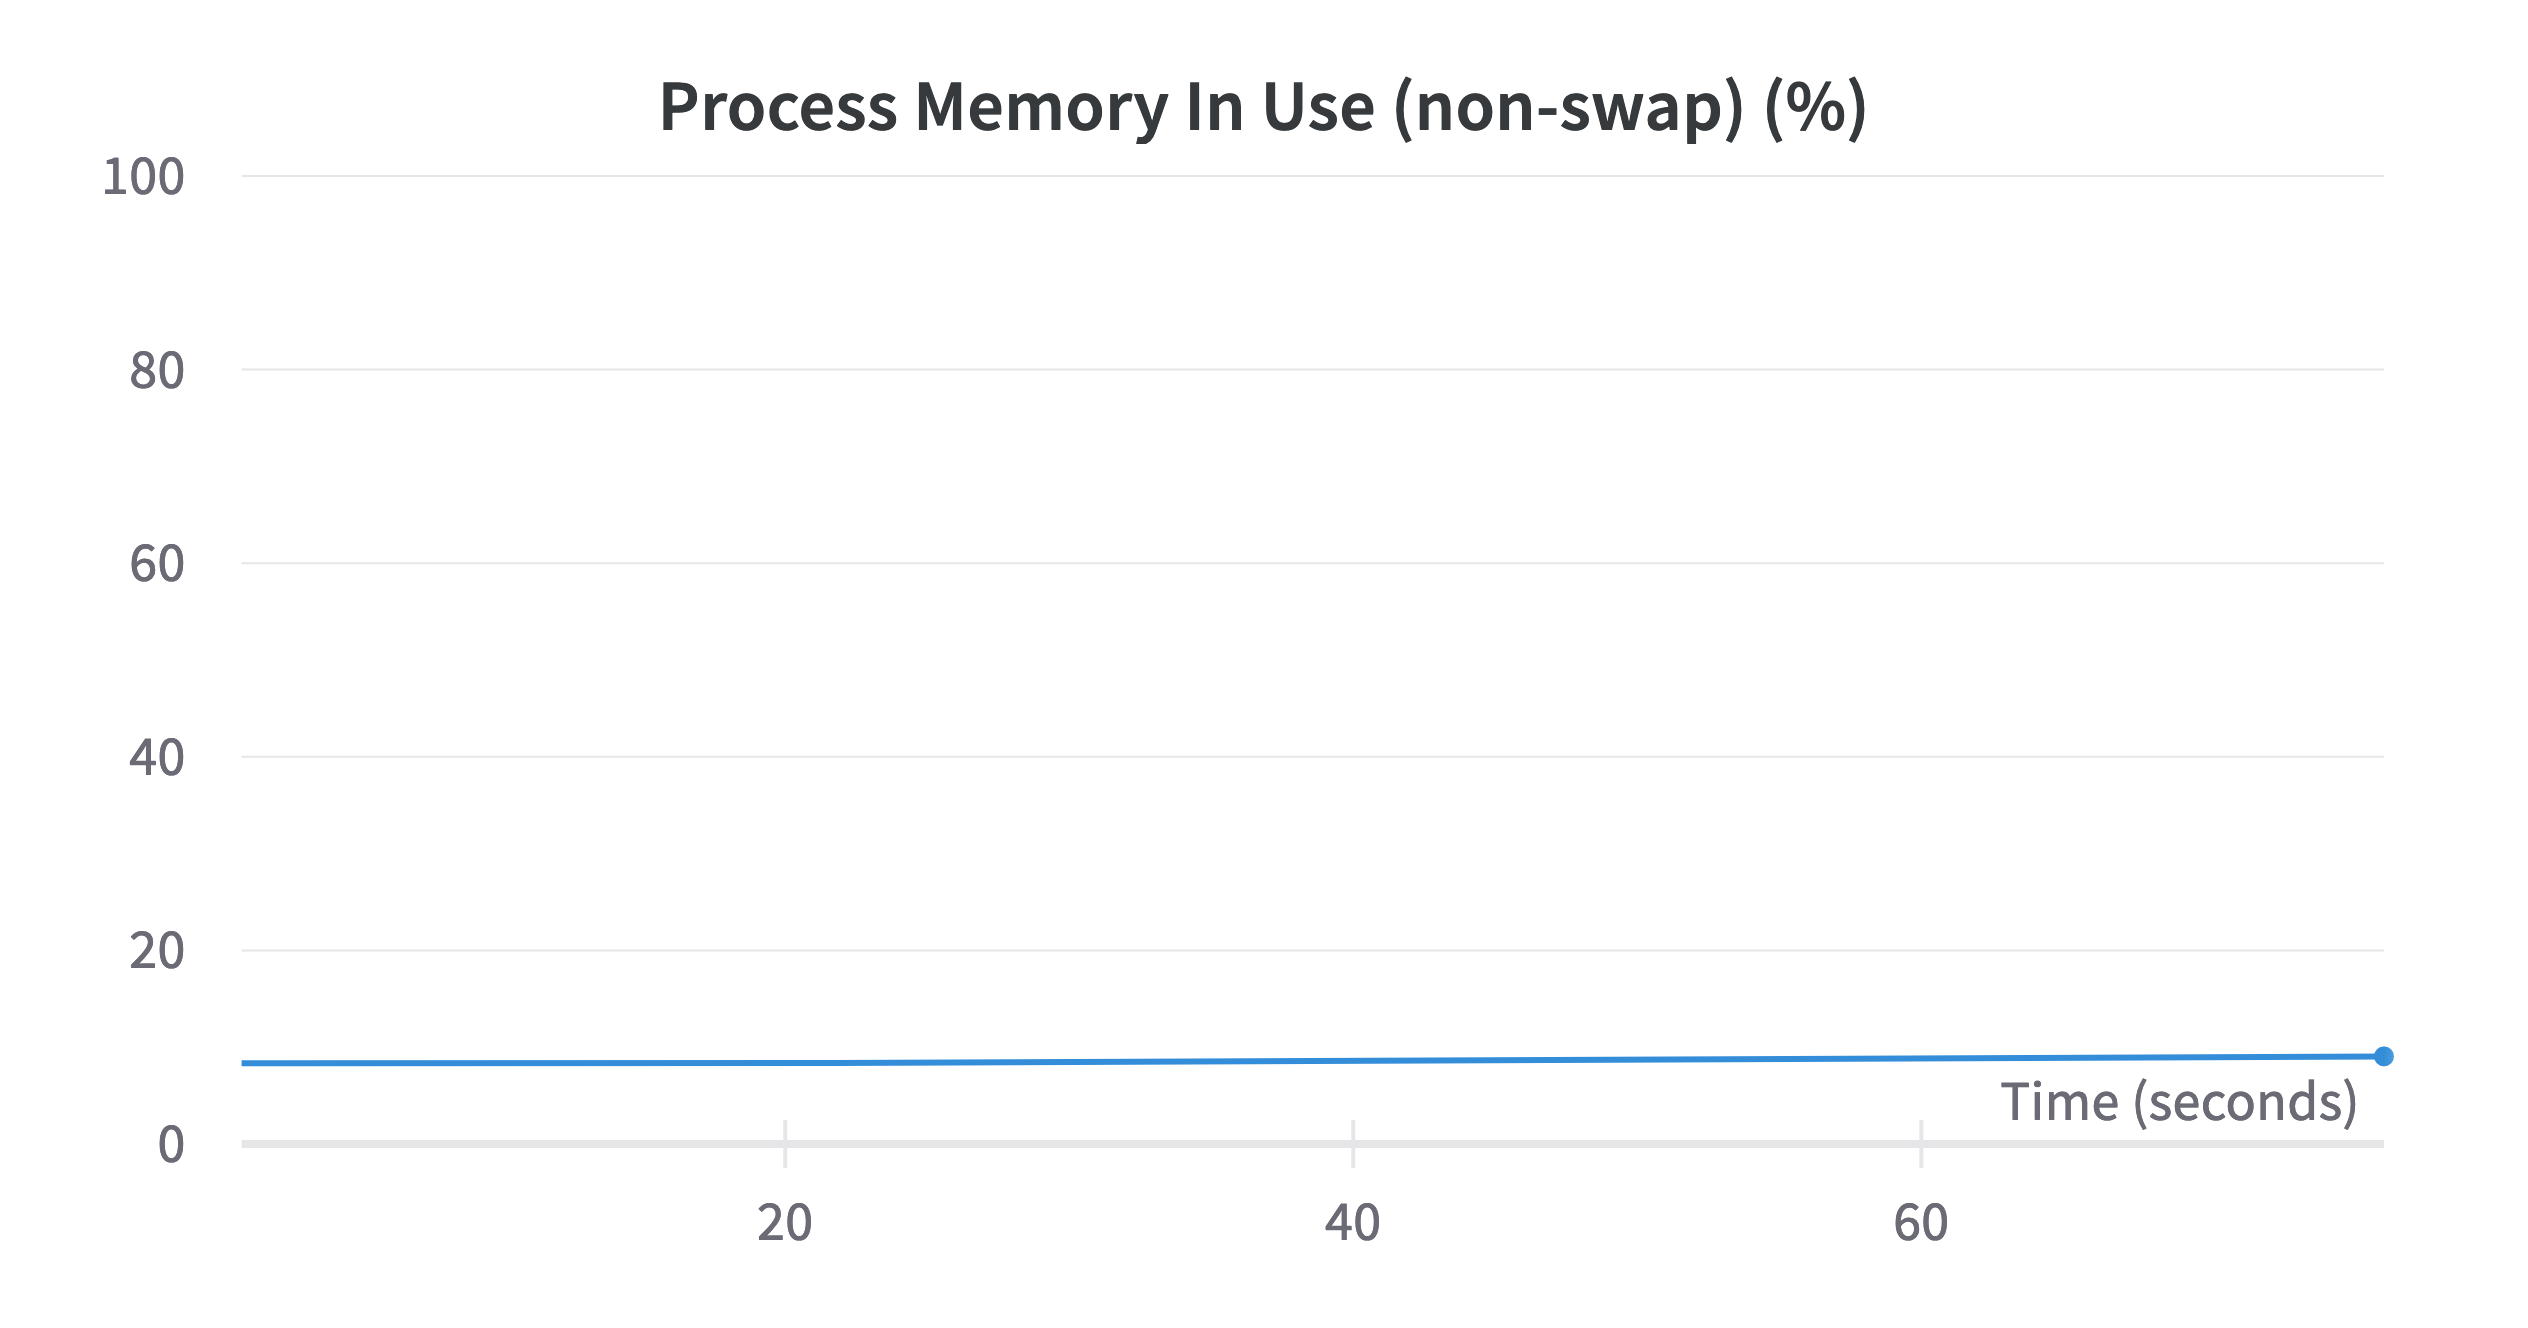
\includegraphics[width=\textwidth]{chapters/3_models/imgs/ufnc/ufcnmemram.png}
	\end{subfigure}\\
	\caption{System resources utilized during the Training phase.}
	\label{fig:ufcnsysusage}
\end{figure}

\begin{algorithm}[H]
	\caption{MLP model Training Algorithm}\label{alg:ufcntraining}
	\begin{algorithmic}
		\Require train/validation datasets; Baseline Neural Network Model

		\State Batch Size $\gets$ 10
		\State Learning Rate $\lambda \gets$ 0.01
		\State Epochs $\gets$ 100
		\State Patience $\gets$ 20
		\State loss $\gets$ L1Loss()
		\State Optimizer $\gets$ Adam Optimizer
		\State
		\For{\textbf{each} epoch \textbf{in} epochs}
		\For{\textbf{each} (batch\_id, before, after, target) \textbf{in} train.next\_batch()}

		\State train\_prediction $\gets$ model(before, after) \Comment{Model inference}
		\State train\_prediction $\gets \frac{\text{train\_prediction} \cdot \sum\text{train\_prediction}}{\sum target}$ \Comment{Area normalization}
		\State train\_loss $\gets$ loss(train\_prediction, target)
		\State Optimizer step
		\State Back Propagation
		\EndFor
		\State stop computing gradient
		\For{\textbf{each} (batch\_id, vbefore, vafter, vtarget) \textbf{in} validation.next\_batch()}
		\State val\_prediction $\gets$ model(vbefore, vafter) \Comment{Model inference}
		\State val\_prediction $\gets \frac{\text{val\_prediction} \cdot \sum\text{val\_prediction}}{\sum vtarget}$ \Comment{Area normalization}
		\State val\_loss $\gets$ loss(val\_prediction, vtarget)
		\EndFor

		\State check for Early Stopping
		\State check for Save Best Result
		\State start computing gradient
		\EndFor
	\end{algorithmic}
\end{algorithm}



\section{RNN based model Evaluation}
From the graphs shown in Figure~\ref{fig:grruntraining},
we can see that the training phase was successful,
and after an initial descent, the loss values remained relatively
constant without displaying any abnormal trends.
The statistics presented in Figure~\ref{fig:grrunsysusage} reveal
that the machine at our disposal was not fully utilized,
suggesting that this architecture can be trained and used on
less powerful computers than the one we have.
Additionally, the model appears to be very lightweight, both in terms
of the relatively small number of parameters and its weight,
which doesn't exceed 400~KB.


\begin{table}[H]
	\begin{center}
		\begin{tabular}[c]{l|l|l}
			%\cline{2-4}
			\multicolumn{1}{c|}{\textbf{Gap Period}} &
			\multicolumn{1}{c|}{\textbf{MAE (kW)}}   &
			\multicolumn{1}{c}{\textbf{R}$^2$}                     \\
			\hline

			02-04 to 05-04                           & 4.72 & 0.96 \\
			04-04 to 04-04                           & 3.60 & 0.93 \\
			12-04 to 14-04                           & 6.61 & 0.96
			% 06-04 to 07-04 & 20.07 & 0.62 &1293.53&50.70&1293.53&25.22 \\
		\end{tabular}
	\end{center}
	\caption{The table displays the values of MAE (Mean Absolute Error) and the R$^2$ (R-squared) index applied to the model predictions shown in Figures~\ref{fig:grrunevalplots}.}
	%La tabella mostra i valori del MAE e dell'indice R$^2$ applicate alle predizioni del modello mostrate nelle Figure~\ref{fig:ufcnevalbelli} e \ref{fig:ufcnevalbrutti}.}\label{tab:dfsplit}
\end{table}

\begin{table}[H]
	\begin{minipage}[t]{.45\textwidth}
		\begin{center}
			\begin{tabular}[c]{l|l|l}
				\multicolumn{3}{c}{\textbf{\textit{02-04 to 05-04 Gap}}}       \\
				%\hline
				               & \multicolumn{1}{c|}{\textbf{MAE (kW)}} &
				\multicolumn{1}{c}{\textbf{MAPE (\%)}}                         \\
				\hline
				\textbf{Day 1} & 97.03                                  & 1.99 \\
				\textbf{Day 2} & 28.68                                  & 3.22 \\
				\textbf{Day 3} & 69.79                                  & 4.79 \\
				\textbf{Day 4} & 41.65                                  & 1.98
			\end{tabular}
			%\caption{}
		\end{center}
	\end{minipage}%
	\hfill
	\begin{minipage}[t]{.45\textwidth}
		\begin{center}
			\begin{tabular}[c]{l|l|l}
				\multicolumn{3}{c}{\textbf{\textit{12-04 to 14-04 Gap}}}       \\
				%\hline
				               & \multicolumn{1}{c|}{\textbf{MAE (kW)}} &
				\multicolumn{1}{c}{\textbf{MAPE (\%)}}                         \\
				\hline
				\textbf{Day 1} & 151.93                                 & 2.86 \\
				\textbf{Day 2} & 49.44                                  & 1.01 \\
				\textbf{Day 3} & 111.25                                 & 2.76
			\end{tabular}
			%\caption{}
		\end{center}
	\end{minipage}%
	\vspace{1cm}
	\begin{minipage}{\textwidth}
		\begin{center}
			\begin{tabular}[c]{l|l|l}
				\multicolumn{3}{c}{\textbf{\textit{04-04 to 04-04 Gap}}}       \\
				%\hline
				               & \multicolumn{1}{c|}{\textbf{MAE (kW)}} &
				\multicolumn{1}{c}{\textbf{MAPE (\%)}}                         \\
				\hline
				\textbf{Day 1} & 0.93                                   & 0.06
			\end{tabular}
			%\caption{}
		\end{center}
	\end{minipage}
	\caption{The tables display the Daily MAE and MAPE values related to the graphs shown in Figure~\ref{fig:grrunevalplots}.}
	%Nelle tabelle sono mostrati i valori giornalieri di MAE e MAPE relativi ai grafici mostrati in Figura~\ref{fig:grrunevalplots}.}
\end{table}

%Dai grafici mostrati in Figura~\ref{fig:grruntraining} possiamo vedere come la fase di addestramento
%è andata a buon fine e, dopo una parte iniziale di discesa, i valori delle loss sono rimasti pressochè costanti e non mostrano andamenti anomali. Dalle statistiche riportate in Figura~\ref{fig:grrunsysusage} possiamo vedere come la macchina a nostra disposizione non è
%stata sfruttata a pieno e questo può portarci a pensare che questa architettura sia allenabile ed
%utilizzabile su computer meno perfromanti di quello a nostra disposizione. Inoltre il modello 
%risulta essere molto leggero, sia per il numero relativamente ridotto di parametri sia per il 
%peso che non supera i 400 KB.

\begin{figure}[H]
	\centering
	\begin{subfigure}{\textwidth}
		\centering
		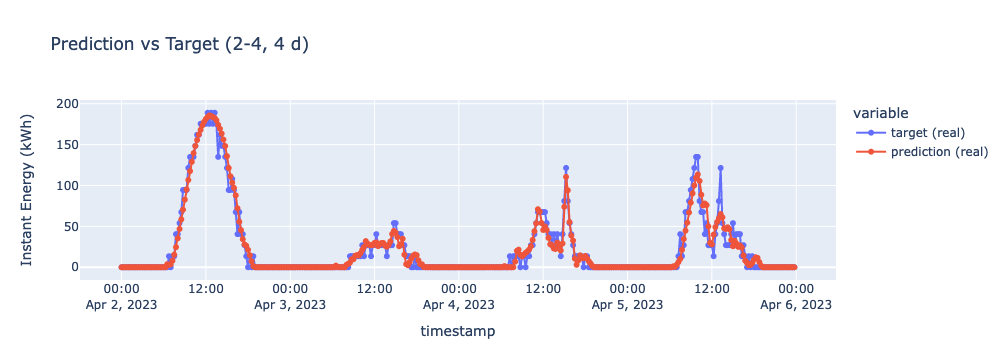
\includegraphics[width=\textwidth]{chapters/3_models/imgs/grrun/eval/grruneval24.png}
		\caption{}
	\end{subfigure}
	\begin{subfigure}{\textwidth}
		\centering
		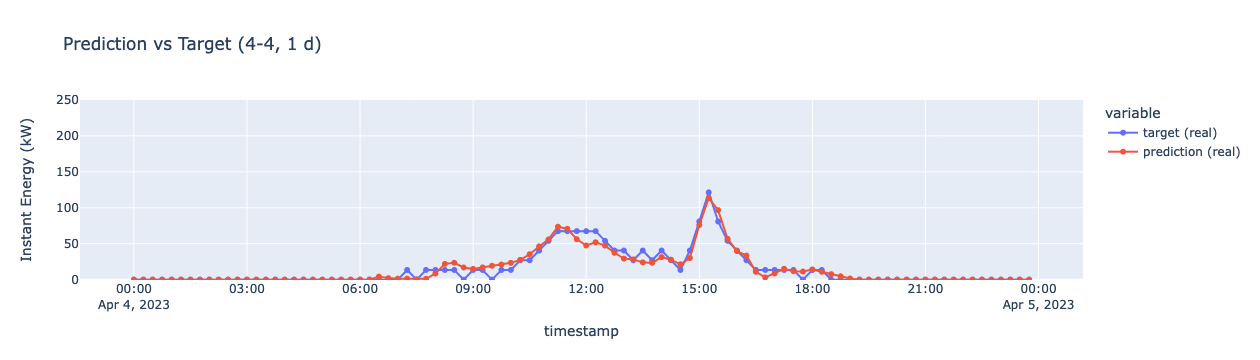
\includegraphics[width=\textwidth]{chapters/3_models/imgs/grrun/eval/grruneval44.png}
		\caption{}
	\end{subfigure}
	\begin{subfigure}{\textwidth}
		\centering
		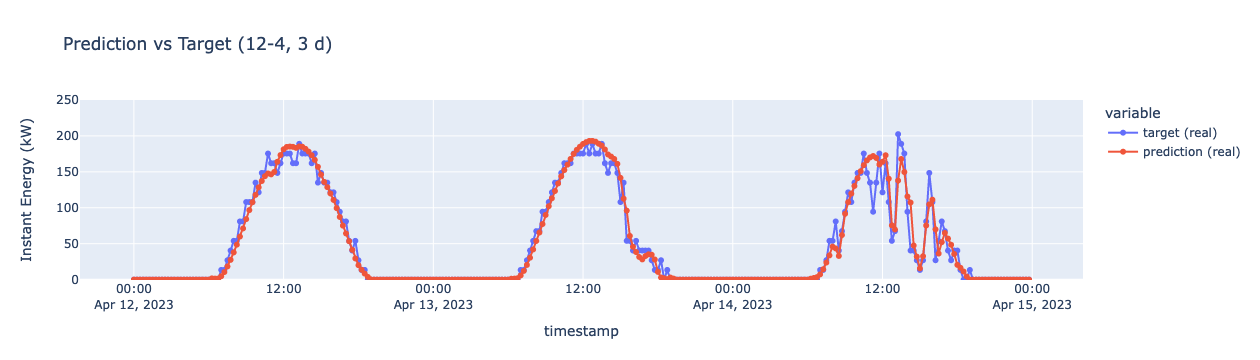
\includegraphics[width=\textwidth]{chapters/3_models/imgs/grrun/eval/grruneval124.png}
		\caption{}
	\end{subfigure}
	\caption{In the figure, three model predictions (in red) are shown alongside the ground truth (in blue) for gaps of varying sizes. These predictions were made using data from the testing dataset.}
	%In figura vengono mostrate 3 predizioni del modello (in rosso) comparate con la ground thorught (in blu) di buchi a dimensione variabile. Queste predizioni sono state effettuate con i dati provenienti dal dataset di Testing.}
	\label{fig:grrunevalplots}
\end{figure}
\newpage
Analyzing some model predictions as shown in
Figure~\ref{fig:grrunevalplots}, we can observe how the real
instant energy production curves (displayed in blue) are
closely approximated by the model (red curves).
The model effectively understands the plant's behavior,
even managing to predict production spikes.
We can also see that energy production is consistently zero during
the night in the predictions, and it adeptly captures the
day/night cycle by gradually reducing production as sunset approaches.

In graph (a), we can see a 4-day gap from 02-04-2023 to 06-04-2023.
The first two days are predicted very well, while in the last part,
we can see that a production spike was not detected.
In graph (b), we can observe a 1-day gap on 04-04-2023. We notice that the overall trend is almost entirely approximated correctly, except for some time intervals around 12:00.
The last graph (c) is related to a 3-day gap, and we can see that the first two days are approximated well, while in the last day, the production spikes are identified but with values not entirely similar to those of the ground truth.
%Analizzando alcune predizioni del modello riportate in Figura~\ref{fig:grrunevalplots} possiamo notare come le curve dell'energia 
%istantanea prodotta realmente (mostrate in blu) vengono approssimate decisamente
%bene dal modello (curve in rosso). Il modello riesce a capire bene il comportamento
%dell'impianto riuscendo anche a prevedere eventuali picchi di produzione.
%Possiamo notare come di notte la produzione di energia nelle predizioni è sempre nulla e come riesce molto bene a comprendere il ciclo giorno/notte
%andando ad azzerare gradualmente la produzione quando si avvicina il tramonto.

%Nel grafico (a) possiamo vedere un buco di 4 giorni che va dal 02-04-2023 al 06-04-2023. I primi due giorni vengono predetti molto bene, mentre nell'ultimo possiamo vedere che un picco di produzione non è stato individuato.
%Nel prolt (b) possiamo apprezzare un buco di 1 giorno, il 04-04-2023.
%Notiamo come l'andamento è quasi del tutto approsiamoto correttamente tranne
%che per alcuni intervalli temporali che si aggirano intorno le 12:00.
%L'ultimo grafico (c) è relativo ad un buco di 3 giorni e possiamo vedere
%come i primi due vengono approssimati bene, mentre nell'ultimo i picchi
%di produzione vengono si individuati ma con valori non del tutto simili
%a quelli della ground truth.

\begin{figure}[H]
	\centering
	\begin{subfigure}{\textwidth}
		\centering
		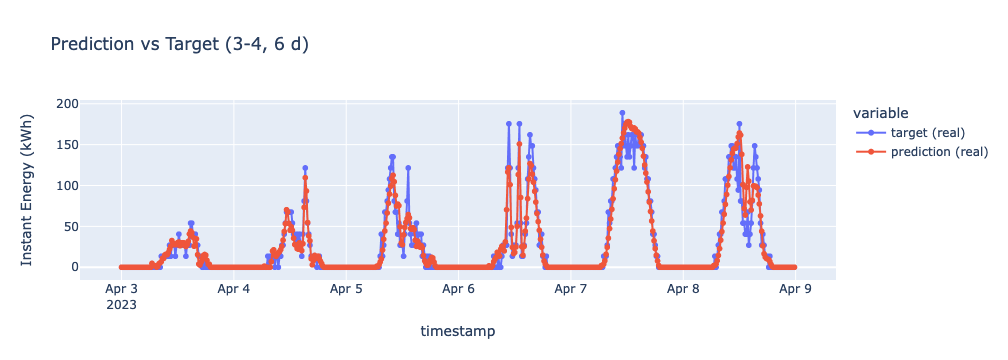
\includegraphics[width=.9\textwidth]{chapters/3_models/imgs/grrun/eval/grruneval6buco.png}
		\caption{}
	\end{subfigure}
	\begin{subfigure}{\textwidth}
		\centering
		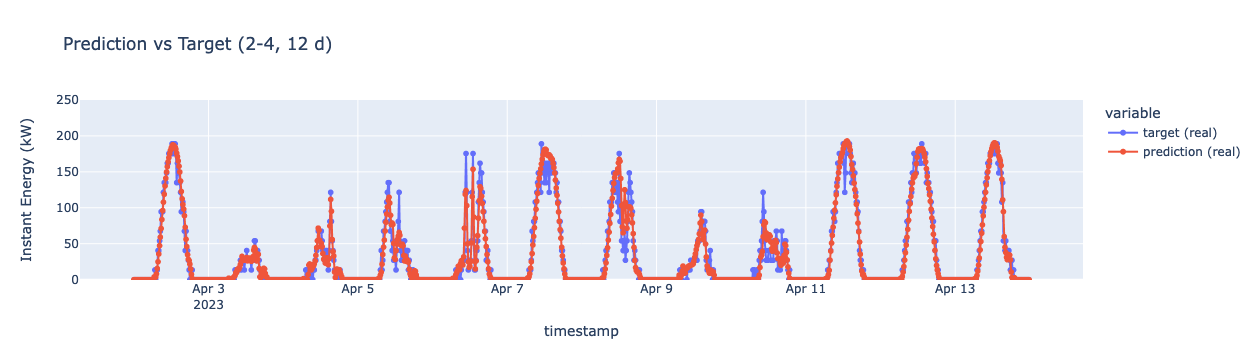
\includegraphics[width=.9\textwidth]{chapters/3_models/imgs/grrun/eval/grruneval12buco.png}
		\caption{}
	\end{subfigure}
	\caption{The graphs depict two model predictions for gaps that exceed the maximum limit of days set during the training phase. The first one (a) shows a 6-day gap, while the second one (b) presents a 12-day gap.}
	%I grafici mostrano due predizioni del modello di buchi con dimensioni che superano il limite massimo di giorni impostati nella fase di training. Il primo (a) mostra un buco di 6 giorni, mentre il secondo (b) uno di 12.}
	\label{fig:grrunevalbucogrande}
\end{figure}

It is interesting to note how the model still performs well even
when presented with gaps that exceed the maximum length set
during training.
In Figure~\ref{fig:grrunevalbucogrande}, two graphs are shown:
(a) represents a 6-day gap (two days longer than the maximum length),
and (b) a 12-day gap.
Given these results, we can conclude that the model can
generalize effectively and predict instant energy production
trends with considerable reliability.


%\'{E} interessante notare come il modello riesce a perforare comunque bene anche se gli vengono passati dei buchi che superano la dimensione massima impostata durante l'addestramento. In Figura~\ref{fig:grrunevalbucogrande} vengono mostrati due grafici, (a) è un buco di 6 giorni (due in più della dimensione massima), mentre (b) è di 12. Dati questi risultati possiamo
%affermare che il modello è in grado di generalizzare molto bene e riuscire
%a predirre l'andamento dell'energia istantanea prodotta con notevole affidabilità.

\begin{table}[H]
	\begin{minipage}[t]{.45\textwidth}
		\begin{center}
			\begin{tabular}[c]{l|l|l}
				\multicolumn{3}{c}{\textbf{\textit{03-04 to 08-04 Gap}}}       \\
				%\hline
				               & \multicolumn{1}{c|}{\textbf{MAE (kW)}} &
				\multicolumn{1}{c}{\textbf{MAPE (\%)}}                         \\
				\hline
				\textbf{Day 1} & 151.93                                 & 2.86 \\
				\textbf{Day 2} & 49.44                                  & 1.01 \\
				\textbf{Day 3} & 111.25                                 & 2.76 \\
				\textbf{Day 4} & 0.93                                   & 0.06 \\
				\textbf{Day 5} & 0.93                                   & 0.06 \\
				\textbf{Day 6} & 0.93                                   & 0.06
			\end{tabular}
			%\caption{}
		\end{center}
	\end{minipage}%
	\hfill
	\begin{minipage}[t]{.45\textwidth}
		\begin{center}
			\begin{tabular}[c]{l|l|l}
				\multicolumn{3}{c}{\textbf{\textit{02-04 to 13-04 Gap}}}        \\
				%\hline
				                & \multicolumn{1}{c|}{\textbf{MAE (kW)}} &
				\multicolumn{1}{c}{\textbf{MAPE (\%)}}                          \\
				\hline
				\textbf{Day 1}  & 148.45                                 & 3.04 \\
				\textbf{Day 2}  & 38.14                                  & 4.28 \\
				\textbf{Day 3}  & 55.41                                  & 3.80 \\
				\textbf{Day 4}  & 20.26                                  & 0.96 \\
				\textbf{Day 5}  & 104.28                                 & 4.09 \\
				\textbf{Day 6}  & 112.09                                 & 2.18 \\
				\textbf{Day 7}  & 312.26                                 & 8.79 \\
				\textbf{Day 8}  & 47.65                                  & 3.46 \\
				\textbf{Day 9}  & 16.32                                  & 0.99 \\
				\textbf{Day 10} & 23.08                                  & 0.43 \\
				\textbf{Day 11} & 240.66                                 & 4.52 \\
				\textbf{Day 12} & 22.21                                  & 0.45
			\end{tabular}
			%\caption{}
		\end{center}
	\end{minipage}
	\caption{The tables presented refer to the graphs in Figure~\ref{fig:grrunevalbucogrande} and display the corresponding Daily MAE and MAPE metrics.}
	%Le tabelle mostrate fanno riferimento ai grafici in Figura~\ref{fig:grrunevalbucogrande} e mostrano le relative metriche Daily MAE e MAPE.}
	%Nelle tabelle sono mostrati i valori giornalieri di MAE e MAPE relativi ai grafici mostrati in Figura~\ref{fig:grrunevalplots}.}
\end{table}
\section{Final Conclusions}
In conclusion, the models described and evaluated in this work have shown varying degrees of success in predicting the instant energy production curve of the plant during gaps. The Recurrent Neural Network-based model, despite being lightweight and efficient, demonstrated limited ability to generalize and predict production variations effectively. It struggled to capture the possibility of production spikes and had difficulty managing the day/night cycle.

While the Unified Fully Connected Network model showed promise, especially in capturing some of the energy production variations, it, too, had limitations when faced with more complex and variable patterns. Both models displayed difficulties in handling gaps of differing sizes.

Overall, the models provide valuable insights into energy production trends, and their predictability can be useful in certain contexts. However, further model refinement and optimization, along with the introduction of techniques that can handle variable gap sizes and more complex patterns, may be necessary to achieve more accurate and reliable predictions. Additionally, expanding the dataset and applying advanced techniques for time series prediction could contribute to more successful models in the future.